\section{MARS Setup}

\subsection{Installation}


Currently, MARS v1.0 is tested to run on Linux platform. To install MARS:

\subsubsection{Python Installation}
\begin{itemize}
\item wget https://www.python.org/ftp/python/2.7.9/Python-2.7.9.tgz
\item tar -xzvf Python-2.7.9.tgz
\item cd Python-2.7.9
\item ./configure --prefix=[Python installation directory]
\item make
\item make test
\item make install

\end{itemize}


\subsubsection{Installing Required Packages}
\begin{itemize}
\item Check if pip or easy\_install are installed, if not do: 
\begin{itemize}
\item wget https://bootstrap.pypa.io/get-pip.py
\item python get-pip.py
\item wget https://bootstrap.pypa.io/ez\_setup.py $-$o $-$ $|$ python
\item easy\_install pip
\end{itemize}
\item Use pip or easy\_install to install the packages in Table~\ref{tab:modules} (e.g. easy\_install numpy or pip install whoosh):
\begin{table}[h]
\captionsetup{justification=justified,
singlelinecheck=true
}
\small{
\caption{List of python packages used for MARS implementation.
}

\begin{tabular}{|p{1.2in}| p{1.8in}| p{2.7in}|}
\hline 
\textbf{Package} & \textbf{Purpose}  &\textbf{Source}\\ 
\hline 
SQLITE & Data Repository & https://sqlite.org/\\
\hline 
Cherrypy & Multi-threaded python server & http://cherrypy.org/\\
\hline 
Whoosh & Search Engine & https://pypi.python.org/pypi/Whoosh/\\
\hline 
Pyparsing & Parser Generator & http://pyparsing.wikispaces.com/\\
\hline 
Bottle Framework & Rest API & http://bottlepy.org/docs/dev/\\
\hline 
MPipe & User-defined Workflows & http://vmlaker.github.io/mpipe/\\
\hline 
matplotlib  & Data Plotting & http://matplotlib.org/\\
\hline 
pythonds & Internal Data Structures (Stack) & https://pypi.python.org/pypi/pythonds\\
\hline 
requests & Send/Receive HTTP Requests & http://docs.python-requests.org/en/master/\\
\hline 
NumPy & Data Analysis & http://www.numpy.org/\\
\hline
NetworkX & Network Structure Measures & https://networkx.github.io/\\
\hline
\end{tabular}
\label{tab:modules}
}
\end{table}
\end{itemize}	


\subsubsection{Downloading MARS Code}
\begin{itemize}
\item Ask Sherif Abdelhamid (sherief@vbi.vt.edu) or Chris Kuhlman(ckuhlman@vbi.vt.edu) to be added to git project (https://ndsslgit.vbi.vt.edu/software-contagion-services/network-services)
\item enter git clone https://ndsslgit.vbi.vt.edu/software-contagion-services/network-services.git
\item cd network-services
\item check the main directories v1 and v2. Each directory has two sub-directories src (code) and doc (manual).
\item v1.0 codes resides under v1/code sub-directory.
\item Copy database file into database directory of your choice (This is a database directory that you created or have access permission to it. Please make sure that it doesn't contain a database file with the same name). \\
scp username@edisondev.vbi.vt.edu:/home/sipcinet/edison/graphservices/database/Edison2.db [database directory]
\end{itemize}

\subsubsection{configuring MARS services}
\begin{itemize}
\item go to [code directory]/v1/src/code
\item check and edit (if needed) the properties:
\begin{itemize}
\item server: name of the python server used. Currently, set to cherrypy, a multithreaded server written python.
\item host: server IP address that will host MARS. It can be set to localhost. 
\item port: list of port numbers that will be used. Each port number is in a separate line. Two services can not share the same port. Make sure when add port to the config file that only one service can use at a time.
\item database: the database directory.
\item index1: location where property queries are indexed on the file system.
\item index2: location where seed queries are indexed on the file system.
\item query: directory where query results are stored on the file system.
\item graph: directory for MARS graphs.
\item code: the directory that contains the services code and the stand-alone executable codes that compute measures on networks.  These codes can be C, C++, Python, Perl, or codes written in any other language.  These are called by the measure service in MARS v2. 

\end{itemize}
\end{itemize}

\subsubsection{Starting MARS Services on edisondev}
Note: the same steps can be done on other VMs, as long as the user has the required permissions and access rights.
\begin{itemize}
\item sudo su - sipcinet
\item export PATH=[python installation directory]:\$PATH
\item go to [code directory]/v1/src/code
\item enter python query\_service.py \&
\end{itemize}




\subsubsection{Starting MARS Services on edison VM (edison.vbi.vt.edu)}
(Note: the same steps can be performed on other VMs as long as the correct directories are provided)
\begin{itemize}
\item sudo su - sip
\item export PATH=[python installation directory]:\$PATH
\item go to [code directory]/v1/src/code
\item enter python query\_service.py \&
\end{itemize}


\subsubsection{Stopping MARS Services}
\begin{itemize}
\item ps ax $|$ grep python [Retrieve python process PID]
\item kill $-$9 PID

\end{itemize}

\subsubsection{Create index for Network Query Search Service}

\begin{itemize}
\item go to [code directory]/v1/src/code
\item enter python create\_index.py [This will create two indexes, for the property and seed type queries]. The indexes directories are specified in the mars.config file as index1 and index2.
\end{itemize}




\subsection{Contribution steps}

To start contributing to MARS repository, please follow these steps:
\begin{itemize}
\item Create a new branch and switch to it [git checkout $-$b [name\_of\_your\_new\_branch]. Name of branch should begin with class type:
\begin{itemize}
\item Feature, if user is adding a new feature for MARS.
\item Bug-fix, if user updating current code to fix a bug.
\item Enhancement, if user is updating current code for code optimization or performance enhancement.
\end{itemize} 

\item Commit the changes with a  descriptive message. [git commit -m "Commit message"]. 
\item Create a new remote for your branch [git remote add [name\_of\_your\_remote]].
\item Push the branch to the remote repository [git push [name\_of\_your\_new\_remote] [name\_of\_your\_new\_branch]].
\item Create a merge request using https://ndsslgit.vbi.vt.edu, as shown in Figure~\ref{fig:merge-request}. Notify other team members to review.
\item Reviewer will check for merge conflicts.
\item Reviewer merge the new branch with master.

\begin{figure}[H]
\centering
%\label{fig:ebola-kshell-not-effective}
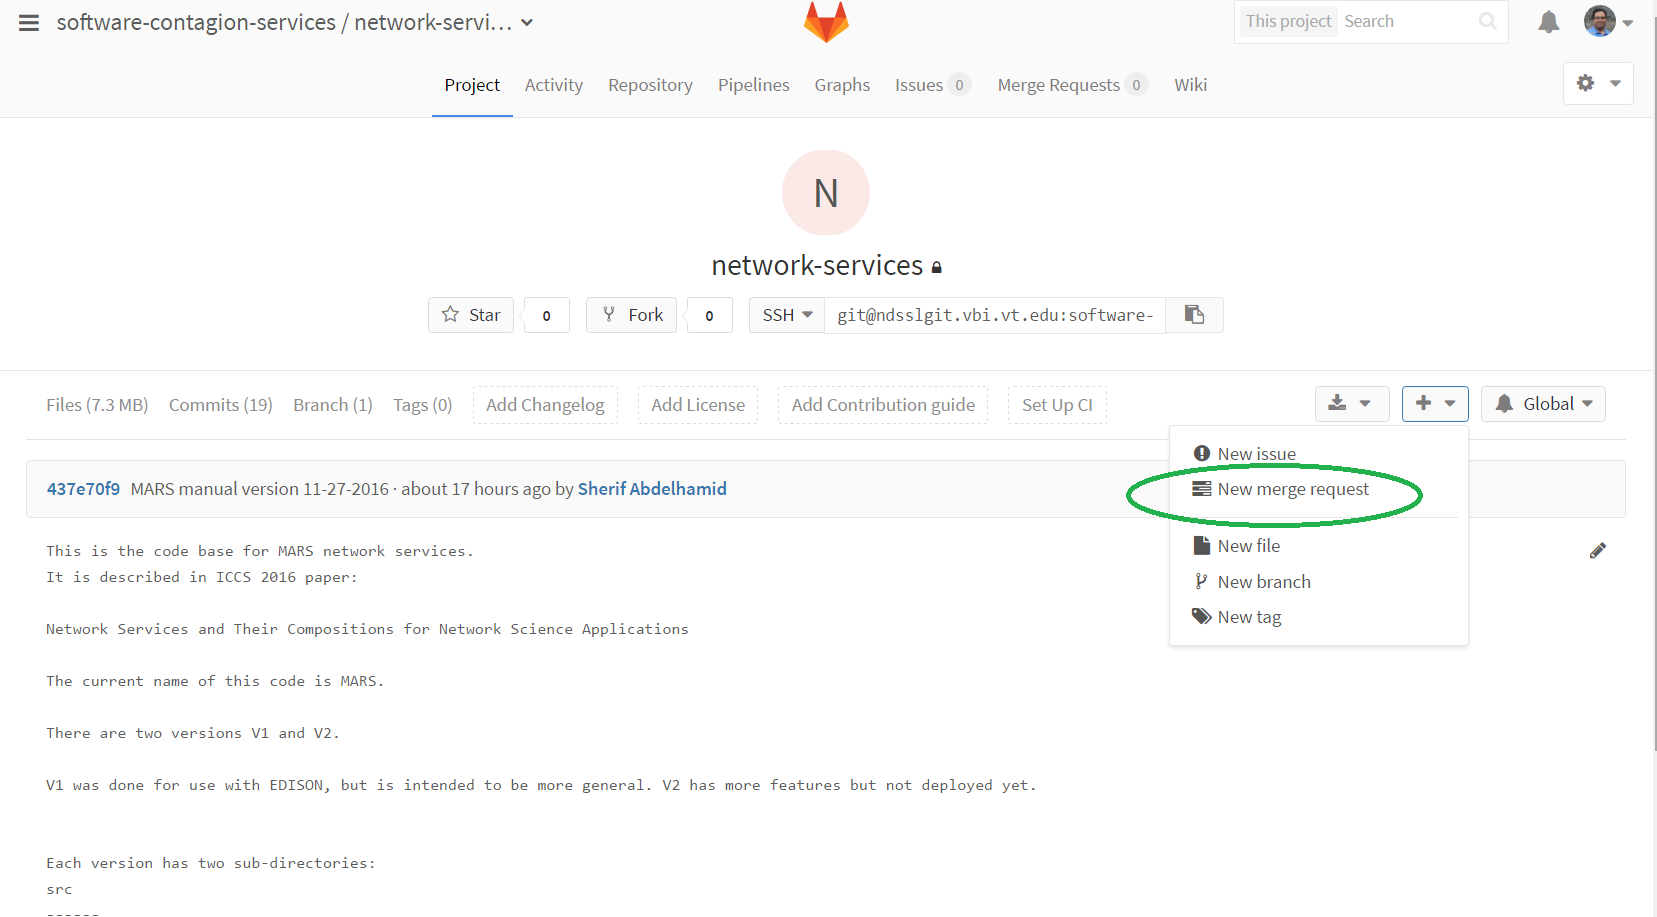
\includegraphics[trim = 0.0in 0.0in 0.0in 0.0in,scale=0.55]{merge-request}
\caption{
Creating a merge request using Web-based interface of ndsslgit.
}   %   
\label{fig:merge-request}
\end{figure}

\end{itemize}



